\newpage
\section{Geometry and Adding Complex Numbers}\label{A:complexAddition}


Let's think about the geometry of adding complex numbers. We won't be
alone on our journey---Louie Llama\index{Louie Llama} is here to help
us out:
\[
\begin{tabular}{ccc}

\includegraphics[scale=.5]{../graphics/llama.pdf} & \qquad $\leftrightsquigarrow$\qquad& 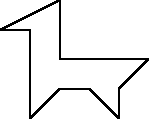
\includegraphics{../graphics/llamaPlot.pdf}\\
Louie Llama & & how we'll draw him
\end{tabular}
\]

\begin{prob} 
Here's Louie Llama hanging out near the point $0$ in the complex
plane. Add $4+4i$ to him. Make a table and show in the plane below what happens.
\[
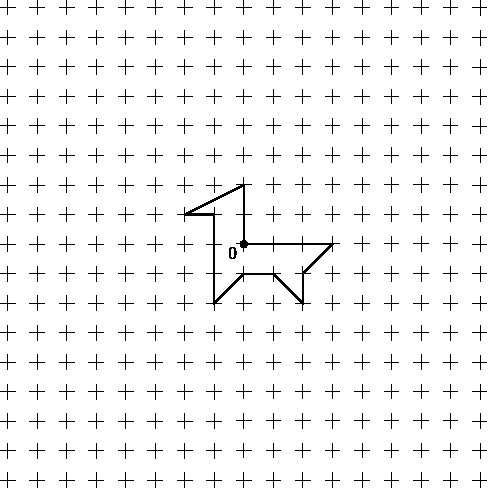
\includegraphics{../graphics/complexAdd.pdf}
\]
\end{prob}

\begin{prob}
Explain what it means to ``add'' a complex number to Louie
Llama. Describe the process(es) used when doing this.
\end{prob}


\begin{prob} 
Put Louie Llama back where he started, now add $1-5i$ to him.  Make a
table and show what happens in the plane.
\end{prob}


\begin{prob} 
Geometrically speaking, what does it mean to ``add'' complex numbers?
\end{prob}
